%% ============================================================
%% HPO Assignment 1 — 2-Page Report
%% RWTH Aachen University | Chair for AI Methodology
%% Prof. Dr. Holger Hoos
%%
%% INSTRUCTIONS FOR SUBMISSION:
%%   Replace this preamble (everything before \begin{document})
%%   with the preamble from the Moodle LaTeX template.
%%   The body content below is ready to use as-is.
%%   Do NOT change font size or margins (assignment constraint).
%% ============================================================

\documentclass[10pt,twocolumn,a4paper]{article}

\usepackage[top=2.5cm,bottom=2.5cm,left=2cm,right=2cm]{geometry}
\usepackage{times}
\usepackage{booktabs}
\usepackage{graphicx}
\usepackage{amsmath}
\usepackage{microtype}
\usepackage[numbers,compress]{natbib}
\usepackage[colorlinks=true,linkcolor=black,citecolor=black,urlcolor=black]{hyperref}

\setlength{\columnsep}{0.6cm}
\bibliographystyle{abbrvnat}

\title{\textbf{Hyperparameter Optimisation: A Comparative Study of\\
       Five Algorithms on YAHPO Gym Benchmarks}}

\author{Anonymous\\
        \small RWTH Aachen University\\
        \small Hyperparameter Optimisation for Machine Learning --- Assignment~1}

\date{}

% ============================================================
\begin{document}
\maketitle
\thispagestyle{empty}

% ---- Introduction ------------------------------------------
\section{Introduction}

Hyperparameter optimisation (HPO) is a fundamental problem in machine learning:
given a learning algorithm and a task, find the configuration of its
hyperparameters that maximises predictive performance.
We evaluate five HPO strategies --- Random Search (RS), Grid Search (GS),
Successive Halving (SH), Hyperband (HB), and Bayesian Optimisation (BO) ---
on two multi-fidelity benchmarks from YAHPO Gym~\cite{pfisterer2022yahpo}:
NB301, a neural architecture search problem on CIFAR-10, and
rbv2\_xgboost, an XGBoost hyperparameter tuning problem.
Our results show that HB achieves the best final performance on the
high-dimensional categorical NB301 space, while multi-fidelity methods
(SH, HB) exhibit a pronounced early-incumbent advantage on rbv2\_xgboost
due to the high correlation between cheap and expensive evaluations.

% ---- Methods -----------------------------------------------
\section{Methods}

\textbf{Random Search (RS)} samples configurations uniformly at random and
evaluates each at maximum fidelity~\cite{bergstra2012random}.
It does not learn from observations and serves as the baseline.

\textbf{Grid Search (GS)} exhaustively evaluates a finite discretisation
of the search space, using 5 evenly-spaced points per continuous dimension
and all choices for categorical dimensions; when the resulting grid exceeds
10{,}000 configurations (as in the 34-dimensional categorical NB301 space),
configurations are drawn uniformly from the per-dimension grids.
GS does not adapt to observed results.

\textbf{Successive Halving (SH)}~\cite{jamieson2016non} is a multi-fidelity
algorithm that begins with $n$ random configurations at minimum budget $r_\mathrm{min}$,
evaluates all, keeps the top $\lfloor n/\eta \rfloor$, and promotes them
to budget $r_\mathrm{min}\cdot\eta$, repeating until one configuration
reaches maximum budget $r_\mathrm{max}$.
We use $\eta=3$ and $n = \lceil \eta^{s_\mathrm{max}+1}/(s_\mathrm{max}+1) \rceil$,
where $s_\mathrm{max} = \lfloor \log_\eta(r_\mathrm{max}/r_\mathrm{min}) \rfloor$.

\textbf{Hyperband (HB)}~\cite{li2018hyperband} addresses SH's sensitivity to the
initial choice of $n$ by running $s_\mathrm{max}+1$ parallel brackets of SH, each
with a different $(n_s, r_s)$ trade-off derived from the formula
$n_s = \lceil (B/r_\mathrm{max}) \cdot \eta^s/(s+1) \rceil$,
$r_s = r_\mathrm{max} \cdot \eta^{-s}$.
The most exploratory bracket ($s{=}s_\mathrm{max}$) evaluates many configurations
cheaply; the least exploratory ($s{=}0$) is equivalent to RS at full budget.

\textbf{Bayesian Optimisation (BO)}~\cite{snoek2012practical} fits a
Gaussian Process (GP) surrogate with a Mat\'{e}rn-5/2 + WhiteKernel to all
observations and selects the next configuration by maximising Expected Improvement (EI).
We implement both EI and its optimisation from scratch using NumPy only:
after 5 random warm-start evaluations, BO evaluates EI for 1{,}000 random
candidates per iteration and returns the best.
BO always evaluates at maximum fidelity; the Mat\'{e}rn-5/2 kernel is chosen
for its balance of smoothness and flexibility~\cite{snoek2012practical}.

% ---- Experimental Setup ------------------------------------
\section{Experimental Setup}

We benchmark all algorithms on two YAHPO Gym scenarios:
(1)~\textbf{NB301 / CIFAR-10}: fidelity = training epochs
    ($r_\mathrm{min}{=}1$, $r_\mathrm{max}{=}98$), metric = validation accuracy;
(2)~\textbf{rbv2\_xgboost / instance 16}: fidelity = training-set fraction
    ($r_\mathrm{min}$ and $r_\mathrm{max}$ read from benchmark metadata),
    metric = accuracy.
Each algorithm receives the same total budget of $B = 50 \times r_\mathrm{max}$
fidelity units, giving RS and BO approximately 50 full-fidelity evaluations,
while SH and HB can explore more configurations cheaply within the same budget.
Budget is measured in fidelity units consumed --- the standard comparison
protocol for multi-fidelity HPO~\cite{li2018hyperband}.
Hyperparameter spaces are accessed via ConfigSpace without the forbidden
methods (\texttt{sample\_configuration}, \texttt{get\_array},
\texttt{generate\_grid}); all sampling is implemented manually.
All experiments are repeated for 10 independent random seeds;
we report mean $\pm$ standard deviation of the best incumbent found.

% ---- Results -----------------------------------------------
\section{Results}

\begin{table}[t]
  \centering
  \caption{Final incumbent performance (mean $\pm$ std over 10 seeds).
           Best per benchmark in \textbf{bold}.}
  \label{tab:results}
  \setlength{\tabcolsep}{4pt}
  \small
  \begin{tabular}{lcc}
    \toprule
    \textbf{Algorithm} & \textbf{NB301} & \textbf{rbv2\_xgb} \\
                       & val\_accuracy  & accuracy \\
    \midrule
    Random Search      & $93.73 \pm 0.17$ & $0.962 \pm 0.005$ \\
    Grid Search        & $93.71 \pm 0.18$ & $0.963 \pm 0.010$ \\
    Succ.\ Halving     & $92.79 \pm 0.17$ & $\mathbf{0.968 \pm 0.007}$ \\
    Hyperband          & $\mathbf{94.16 \pm 0.20}$ & $0.967 \pm 0.007$ \\
    Bayesian Opt.      & $94.08 \pm 0.32$ & $0.966 \pm 0.013$ \\
    \bottomrule
  \end{tabular}
\end{table}

Table~\ref{tab:results}, Figure~\ref{fig:incumbent}, and Figure~\ref{fig:boxplot}
summarise our results.

\paragraph{NB301 (CIFAR-10).}
All methods reach approximately $93\%$ validation accuracy within the first 500
budget units (Figure~\ref{fig:incumbent}, left), but thereafter diverge.
HB achieves the highest final accuracy ($94.16 \pm 0.20$), followed closely by BO
($94.08 \pm 0.32$).
RS and GS form a mid-tier baseline (${\approx}93.7\%$), while SH is the
weakest ($92.79 \pm 0.17$).
HB's advantage over SH stems from its bracket portfolio:
a single SH bracket exhausts its initial candidate set and restarts from scratch,
whereas HB concurrently maintains brackets at different fidelity trade-offs,
sustaining exploration of promising regions throughout the budget.
BO's high variance ($\pm 0.32$, Figure~\ref{fig:boxplot}) reflects the
difficulty of fitting a GP to NB301's 34-dimensional categorical space ---
the one-hot encoding produces a 234-dimensional input, degrading surrogate
quality under the curse of dimensionality.
RS and GS perform nearly identically, confirming that non-adaptive methods
cannot exploit evaluation history regardless of the search strategy.

\paragraph{rbv2\_xgboost (Dataset 16).}
Performance differences are smaller overall (range $0.962$--$0.968$),
but the incumbent curves (Figure~\ref{fig:incumbent}, right) reveal a
pronounced early advantage for multi-fidelity methods:
SH and HB reach $\approx 0.96$ accuracy within only 10 budget units,
while RS, GS, and BO require 20--30 units to reach comparable performance.
This advantage arises because cheap low-fidelity evaluations (small training
fractions) are highly informative for XGBoost --- the ranking of configurations
is stable across fidelity levels, so SH and HB identify and promote the best
candidates early.
By budget exhaustion all five methods converge to similar final accuracy,
consistent with this benchmark's smooth, well-conditioned objective surface.

\begin{figure}[t]
  \centering
  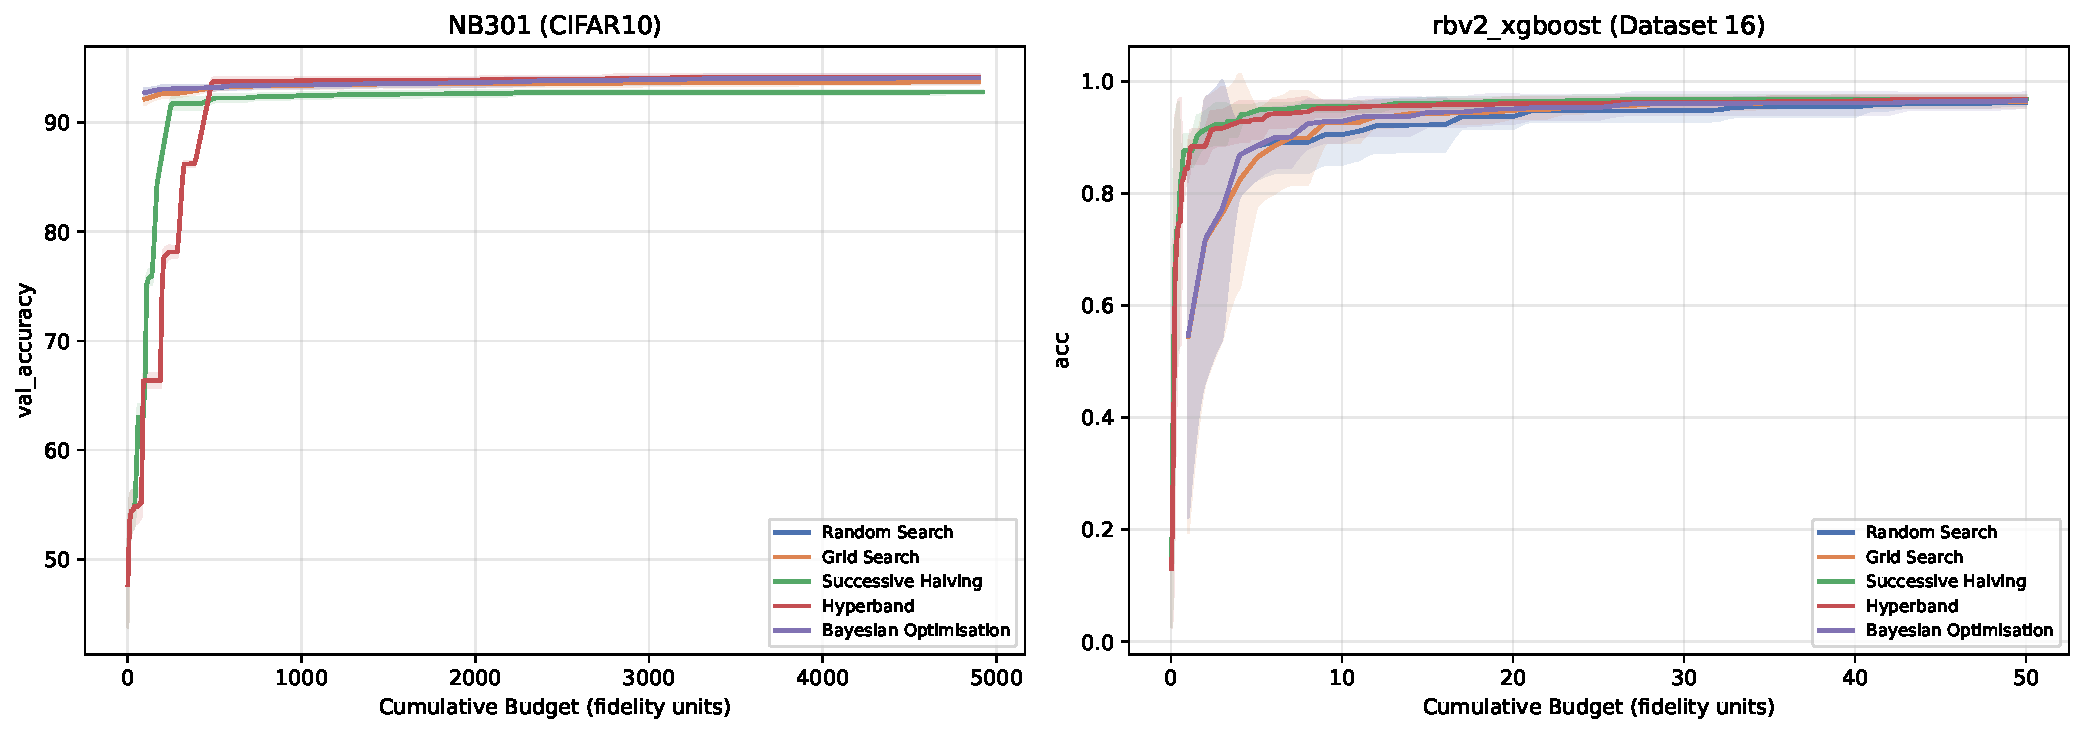
\includegraphics[width=\columnwidth]{../figures/incumbent_curves.pdf}
  \caption{Incumbent curves (mean $\pm$ 1 std over 10 seeds).
           Left: NB301/CIFAR-10. Right: rbv2\_xgboost/instance 16.
           Budget is measured in fidelity units consumed.}
  \label{fig:incumbent}
\end{figure}

\begin{figure}[t]
  \centering
  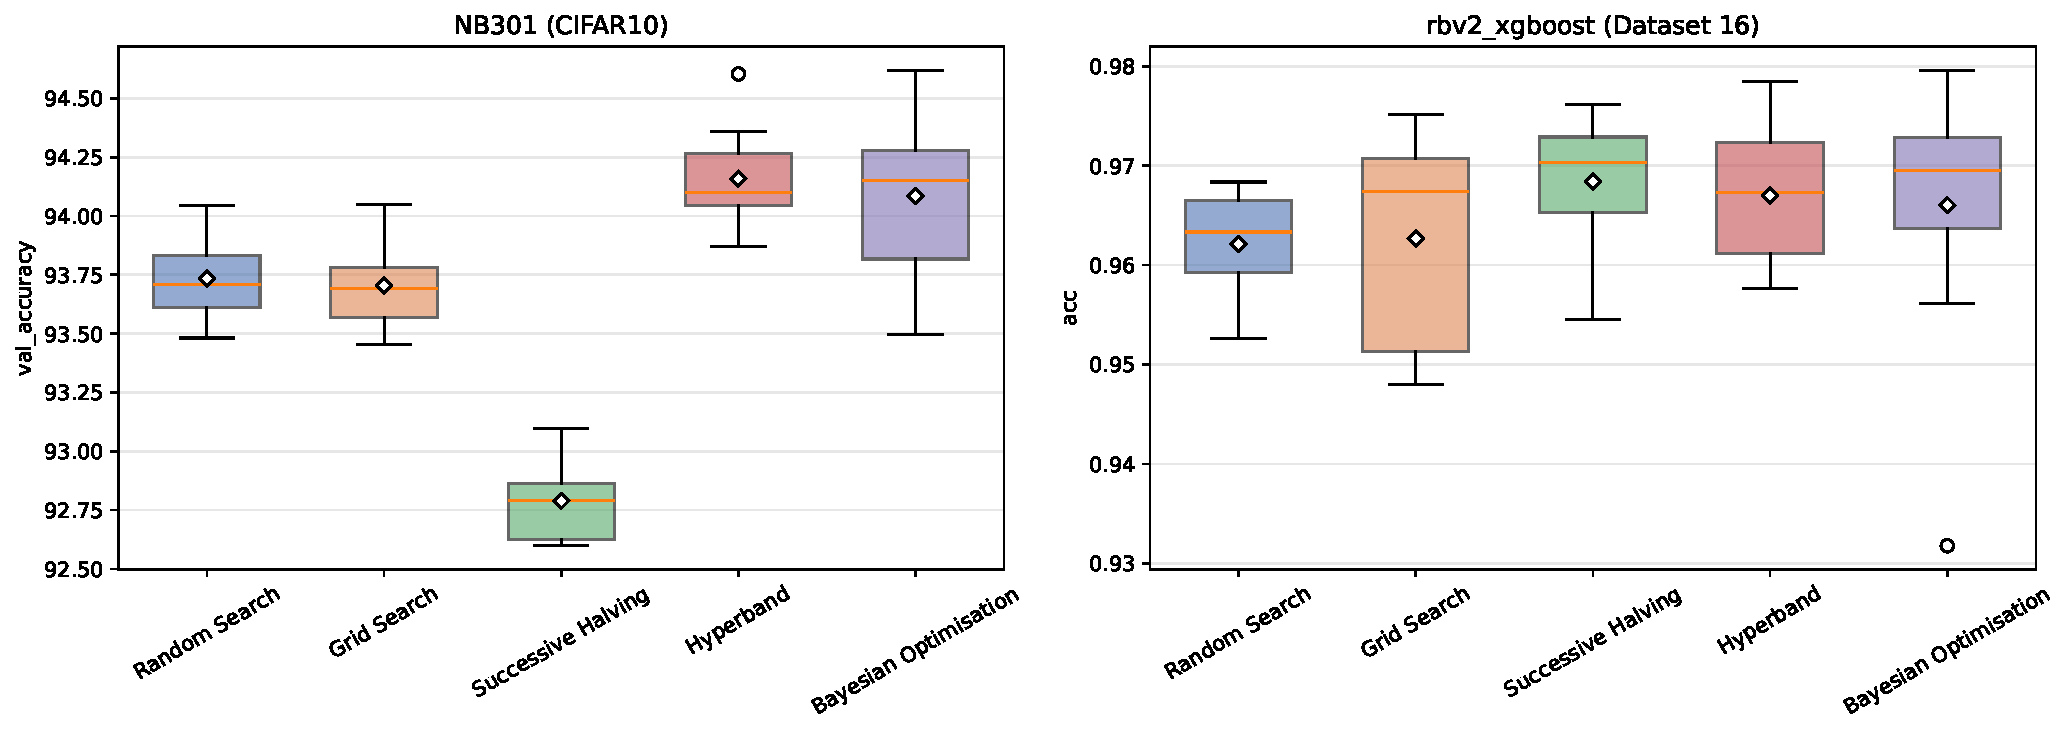
\includegraphics[width=\columnwidth]{../figures/final_performance.pdf}
  \caption{Distribution of final incumbent across seeds.
           HB achieves the highest median on NB301; SH and HB tie on rbv2.
           BO exhibits the largest spread on NB301 (outlier visible).}
  \label{fig:boxplot}
\end{figure}

% ---- Conclusions -------------------------------------------
\section{Conclusions}

HB is the most robust algorithm across both benchmarks, achieving the
highest accuracy on NB301 and matching SH on rbv2\_xgboost,
with consistently low variance.
Its bracket portfolio effectively amortises the risk of a suboptimal
fidelity trade-off --- the key advantage over a single SH bracket.
BO is competitive on NB301 but its GP surrogate degrades in
high-dimensional categorical spaces, yielding higher variance.
Multi-fidelity methods (SH, HB) are particularly effective when cheap
proxy evaluations are informative, as demonstrated by their early-incumbent
advantage on rbv2\_xgboost.
RS and GS are reliable but suboptimal baselines; practitioners should
prefer HB or BO for any budget exceeding a few dozen full evaluations.

% ---- References --------------------------------------------
\begin{thebibliography}{9}

\bibitem{bergstra2012random}
J.~Bergstra and Y.~Bengio.
\newblock Random search for hyper-parameter optimization.
\newblock \emph{Journal of Machine Learning Research}, 13:281--305, 2012.

\bibitem{jamieson2016non}
K.~Jamieson and A.~Talwalkar.
\newblock Non-stochastic best arm identification and hyperparameter optimization.
\newblock In \emph{AISTATS}, 2016.

\bibitem{li2018hyperband}
L.~Li, K.~Jamieson, G.~DeSalvo, A.~Rostamizadeh, and A.~Talwalkar.
\newblock Hyperband: A novel bandit-based approach to hyperparameter optimization.
\newblock \emph{Journal of Machine Learning Research}, 18(185):1--52, 2018.

\bibitem{snoek2012practical}
J.~Snoek, H.~Larochelle, and R.~P. Adams.
\newblock Practical Bayesian optimization of machine learning algorithms.
\newblock In \emph{NeurIPS}, 2012.

\bibitem{pfisterer2022yahpo}
F.~Pfisterer, L.~Schneider, J.~Moosbauer, M.~Binder, and B.~Bischl.
\newblock {YAHPO Gym} -- An efficient multi-objective multi-fidelity benchmark
  for hyperparameter optimization.
\newblock In \emph{AutoML Conference}, 2022.

\end{thebibliography}

\end{document}
